%%%%%%%%%%%%%%%%%%%%%%%%%%%%%%%%%%%%%%%%%%%%%%%
%% Introduction aux Systèmes d'exploitation  %%
%%   * Historique                            %%
%%   * Principes fondamentaux                %%
%%   * Grandes classes de systèmes           %%
%%%%%%%%%%%%%%%%%%%%%%%%%%%%%%%%%%%%%%%%%%%%%%%

\title{Systèmes d'exploitation}
\subtitle{Lex et Yacc : partie I (Lex)}

\author{Yves \textsc{Stadler}}\institute{Codasystem, UPV-M}

\date{\today}

\begin{document}


%%
% Page de Titre
%%
\begin{frame}
\titlepage
\end{frame}


%!!!!!!!!!!!!!!!!!!!!!!!!!!!!!!!!!!!!!!!!!
\def\ftitle{Introduction}
\begin{frame}[containsverbatim]{\ftitle}
%_________________________________________
\def\blocktitle{Lexical analyser}
\begin{block}{\blocktitle}
\begin{itemize}
\item Programme qui génêre des analyseur lexical
\item Appelle aussi parfois "lexer" ou "parser"
\item Permet de "parser" un fichier, le scanner.
\end{itemize}
\end{block}
%_________________________________________
\def\blocktitle{Historique}
\begin{block}{\blocktitle}
\begin{itemize}
\item Original by AT\&T
\item OpenSource fourni dans OpenSolaris et Plan9 des laboratoires Bell.
\item On utilise maintenant flex (fast lex)
\end{itemize}
\end{block}
\end{frame}


%!!!!!!!!!!!!!!!!!!!!!!!!!!!!!!!!!!!!!!!!!
\def\ftitle{Introduction}
\begin{frame}[containsverbatim]{\ftitle}
%_________________________________________
\def\blocktitle{principe}
\begin{block}{\blocktitle}
\begin{itemize}
\item Écrire une liste d'expression
\item Écrire une liste d'actions 
\item Générer un programme qui va parcourir un fichier et effectue les actions décrites pour les expressions choisies.
\item Le fichier .lex donnera un fichier source à utiliser dans le langage choisi.
\end{itemize}
\end{block}
\end{frame}

%!!!!!!!!!!!!!!!!!!!!!!!!!!!!!!!!!!!!!!!!!
\def\ftitle{Structure d'un fichier Lex}
\begin{frame}[containsverbatim]{\ftitle}
%_________________________________________
\def\blocktitle{Général}
\begin{block}{\blocktitle}
\begin{itemize}
\item \begin{verbatim}Definition section
%%
Rules section
%%
language code section
\end{verbatim}
\item Langage cible : C (pour ce cours)
\item Définition section : permet de donner des instructions pour le fichier source généré
\item Rules section : productions de lex
\item Language code section : code additionnel dans le langage cible.
\item Le fichier aura l'extension .l, .lex la plupart du temps.
\end{itemize}
\end{block}
\end{frame}

%!!!!!!!!!!!!!!!!!!!!!!!!!!!!!!!!!!!!!!!!!
\def\ftitle{Structure d'un fichier Lex}
\begin{frame}[containsverbatim]{\ftitle}
%_________________________________________
\def\blocktitle{Définitions}
\begin{block}{\blocktitle}
\begin{itemize}
\item Définition des macros (\verb!#!define)
\item Includes (stdio.h etc)
\item Options
\item Des commentaires \verb!/* .... */!
\item Des notions non terminales
\end{itemize}
\end{block}
%_________________________________________
\def\blocktitle{Syntaxe}
\begin{block}{\blocktitle}
\begin{itemize}
\item Tous code du langage cible est entouré de \verb!%{! et \verb!}%!
\item Les instructions Lex ne sont pas encadré ainsi
\item Une notion non terminale est une association entre un nom et une expression régulière.
\item \verb!notion expression!
\item \verb!nombre [0-9]+!
\end{itemize}
\end{block}
\end{frame}


%!!!!!!!!!!!!!!!!!!!!!!!!!!!!!!!!!!!!!!!!!
\def\ftitle{Productions}
\begin{frame}[containsverbatim]{\ftitle}
%_________________________________________
\def\blocktitle{Productions}
\begin{block}{\blocktitle}
\begin{itemize}
\item Dire à Lex quoi faire en rencontrant une notion
\item (notion|expression) action
\item Si action est absent, lex recopie les caractères tels quels sur la sortie standard
\item Si il y a plus d'une instruction il faut mettre des \verb!{ }! autour des actions
\item Pas besoin de mettre  \verb!%{! et \verb!}%! pour les actions
\item En revanche on pourra metter entre \verb!%{! et \verb!}%! en début des productions une liste d'instruction que sera incluse dans le code de la fonction générée yylex()
\item Il faut mettre les notions entre accolades
\end{itemize}
\end{block}
\end{frame}


%!!!!!!!!!!!!!!!!!!!!!!!!!!!!!!!!!!!!!!!!!
\begin{frame}[containsverbatim]{\ftitle}
%_________________________________________
\def\blocktitle{Exemple}
\begin{block}{\blocktitle}
\begin{itemize}
\item \begin{verbatim}[0-9]+  {
            /* yytext contient la chaîne matchée */
            printf("Saw an integer: %s\n", yytext);
        }
.       {   /* Ignore all other characters. */   }

\item \begin{verbatim}{nombre}  {
            /* yytext contient la chaîne matchée */
            printf("Saw an integer: %s\n", yytext);
        }
.       {   /* Ignore all other characters. */   }
\end{verbatim}
\end{itemize}
\end{block}
\end{frame}

%!!!!!!!!!!!!!!!!!!!!!!!!!!!!!!!!!!!!!!!!!
\def\ftitle{Code additionnel}
\begin{frame}[containsverbatim]{\ftitle}
%_________________________________________
\def\blocktitle{Principe}

\begin{columns}[c]
\column{0.4\textwidth}
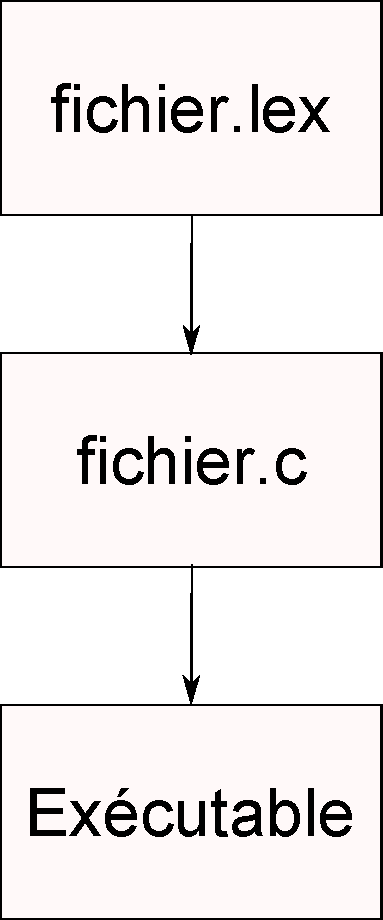
\includegraphics[width=.6\textwidth]{images/chaine.pdf}
\column{.6\textwidth}
\begin{block}{\blocktitle}
\begin{itemize}
\item Lex va générer un fichier C à partir d'un fichier lex
\item Plutôt que de modifier ce fichier pour ajouter le main, on peut l'ajouter dans la partie code additionnel.
\item On peut aussi y écrire d'autre fonctions bien sur!
\end{itemize}
\end{block}
\end{columns}
\end{frame}

%!!!!!!!!!!!!!!!!!!!!!!!!!!!!!!!!!!!!!!!!!
\begin{frame}[containsverbatim]{\ftitle}
%_________________________________________
\def\blocktitle{Syntaxe}
\begin{block}{\blocktitle}
\begin{verbatim}int main(void) {
	/* Du code */
	
	/* On appelle l'analyseur lexical */
	yylex();
	/* Du code */
	return 0;
}

\end{verbatim}
\end{block}
\end{frame}

%!!!!!!!!!!!!!!!!!!!!!!!!!!!!!!!!!!!!!!!!!
\def\ftitle{Options}
\begin{frame}[containsverbatim]{\ftitle}
%_________________________________________
\def\blocktitle{Options disponibles}
\begin{block}{\blocktitle}
\begin{itemize}
\item \verb!%pointer! \verb!%array! pour choisir le type de yytext (pointeur ou tableau externe)
\item \verb!%noyywrap! Par défaut yylex() appelle la fonction yywrap() pour continuer les traitements après avoir détecter une notion.
Cela nous permettra de réaliser des analyse grammaticales. Si il n'y a pas de traitement supplémentaire, on précise cette option.
\end{itemize}
\end{block}
%_________________________________________
\def\blocktitle{Variables speciales}
\begin{block}{\blocktitle}
\begin{itemize}
\item yyin : entrée standard de yylex (défaut: stdin)
\item \verb!yyin = fopen("fichier", "r");!
\item \verb!yytext! la chaîne de caractère mise en correspondance.
\end{itemize}
\end{block}
\end{frame}
\end{document}
